\documentclass[a4paper,12pt]{article}
\usepackage{tikz}
\usetikzlibrary{circuits.logic.US, positioning}
\usepackage[utf8]{inputenc}
\usepackage{amsmath}
\usepackage{geometry}
\geometry{margin=1in}
\usepackage{caption}
\usepackage{subcaption}
\usepackage{xcolor}
\usepackage{fancyhdr}
\usepackage{array}
\usepackage{float}
\usepackage{enumitem}
\definecolor{darkskyblue}{rgb}{0.0, 0.5, 1.0}
\definecolor{skyblue}{RGB}{135, 206, 235}

\geometry{a4paper, top=0.7in, left=1in, right=1in, bottom=1in}

\begin{document}
\pagestyle{empty} % Start with empty page style

\thispagestyle{fancy} % Apply fancy style only to the first page
\fancyhf{} % Clear header and footer
\renewcommand{\headrulewidth}{0pt} % Remove header rule

\fancyhead[L]{% Left header
    
\includegraphics[width=6.5cm, height=1.3cm]{img3.png}
}

\fancyhead[R]{% Right header
    Name: K.Saisusmitha \\
    Batch: COMETFWC018 \\
    Date: 4 July 2025
}

\vspace{1.5cm}
\begin{center}
    {\LARGE \textbf{\textcolor{darkskyblue}{GATE QUESTION\\EC 2010 Q12}}}
\end{center}

\vspace{0.5cm}
\section*{\textcolor{blue}{Question}}

\noindent\textbf{Q.12} For the output \( F \) to be 1 in the logic circuit shown, the input combination should be:

\vspace{1em}

\begin{center}
    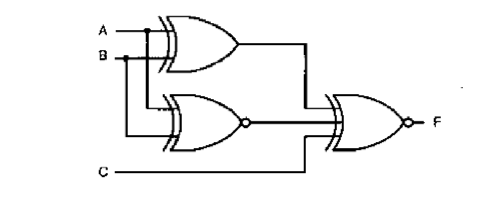
\includegraphics[width=0.45\textwidth]{fpga.png}
\end{center}

\vspace{1em}

\noindent\textbf{Options:}
\begin{enumerate}[label=(\Alph*)]
    \item \( A = 1, B = 1, C = 0 \)
    \item \( A = 1, B = 0, C = 0 \)
    \item \( A = 0, B = 1, C = 0 \)
    \item \( A = 0, B = 0, C = 1 \)
\end{enumerate}

\vspace{1em}

\noindent\textbf{Correct Answer:} \fbox{(A) \( A = 1, B = 1, C = 0 \)}

\vspace{1cm}

\section*{\textcolor{blue}{Explanation}}

From the circuit:

- The first gate is an \textbf{OR gate} with inputs \( A \) and \( B \).
- The second gate is an \textbf{AND gate} with inputs \( B \) and \( C \).
- The output of both gates is fed to another \textbf{OR gate} to get output \( F \).

Let us compute step-by-step for option (A): \( A = 1, B = 1, C = 0 \)

\begin{itemize}
    \item OR gate: \( A + B = 1 + 1 = 1 \)
    \item AND gate: \( B \cdot C = 1 \cdot 0 = 0 \)
    \item Final OR gate: \( 1 + 0 = 1 \Rightarrow F = 1 \)
\end{itemize}

\noindent
Only option (A) gives output \( F = 1 \).

\vspace{0.5em}
\noindent\textbf{Hence, the correct answer is:} \fbox{(A)}

\end{document}
